\documentclass[tikz, border=20pt]{standalone}
\usepackage[utf8]{inputenc}
\usepackage[T5]{fontenc}
\usepackage{lmodern}
\usepackage{xcolor}
\usepackage{graphicx}
\usetikzlibrary{positioning, calc, arrows}

\begin{document}
\begin{tikzpicture}[
  >=stealth,
  font=\sffamily,
  % Khung card nét đứt chuẩn khoa học, chiều cao đồng nhất
  tierCard/.style={
    draw=black,
    dashed,
    line width=1.3pt,
    fill=white,
    rounded corners=6pt,
    inner sep=10pt,
    align=center
  },
  % Nhãn trên mũi tên
  tagText/.style={
    font=\small\bfseries,
    fill=white,
    inner sep=3.5pt,
    rounded corners=2.5pt,
    draw=black!45,
    line width=0.6pt,
    text=black
  },
  arrowThick/.style={
    ->,
    line width=1.8pt,
    draw=black
  },
  biArrowThick/.style={
    <->,
    line width=1.8pt,
    draw=black
  }
]

% ==================== 1. TẦNG 2: THU THẬP & DSP (ĐẶT Ở TRUNG TÂM HÀNG GIỮA) ====================
\node[tierCard, text width=7.0cm, minimum height=7.2cm] (tier2) at (0, 0) {
  {\bfseries\Large TẦNG 2: THU THẬP \& DSP}\\[2pt]
  {\footnotesize\color{black!70} (Sensing \& DSP Tier)}\\[8pt]
  
  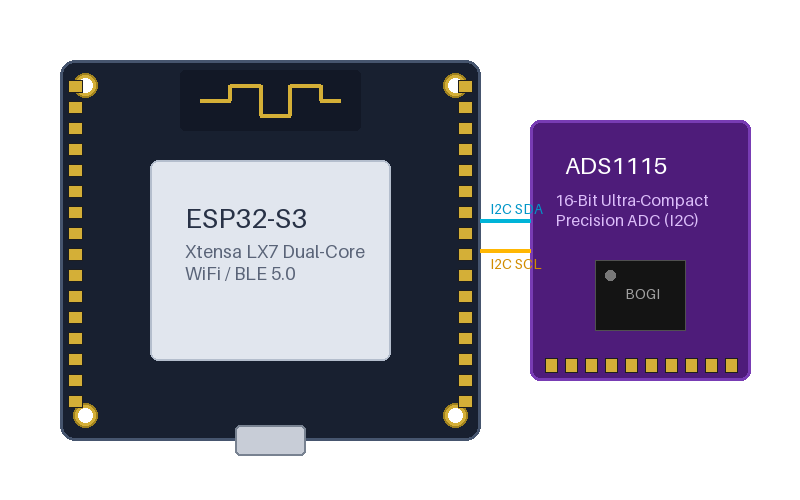
\includegraphics[width=4.8cm, height=2.6cm, keepaspectratio]{assets/controller_ads_board.png}\\[6pt]
  {\bfseries\normalsize ESP32-S3 + ADC ADS1115}\\[2pt]
  {\footnotesize 2 MUX CD74HC4067 (21 kênh $\ge$15Hz)}\\[8pt]
  
  {\bfseries\normalsize Lọc số DSP 2 nhánh \& Bộ chỉ số}\\[2pt]
  {\footnotesize Khử trôi tĩnh $\bullet$ Tính EI -- GAP -- RAL}\\[2pt]
  {\small Thuật toán trợ lực theo nhu cầu (AAN)}
};

% ==================== 2. TẦNG 1 (TRÁI) VÀ TẦNG 3 (PHẢI) CĂN ĐỈNH CHUẨN XÁC VỚI TẦNG 2 ====================
\node[tierCard, text width=6.6cm, minimum height=7.2cm, left=72pt of tier2.north west, anchor=north east] (tier1) {
  {\bfseries\Large TẦNG 1: TẦNG ĐEO}\\[2pt]
  {\footnotesize\color{black!70} (Wearable Physical Tier)}\\[8pt]
  
  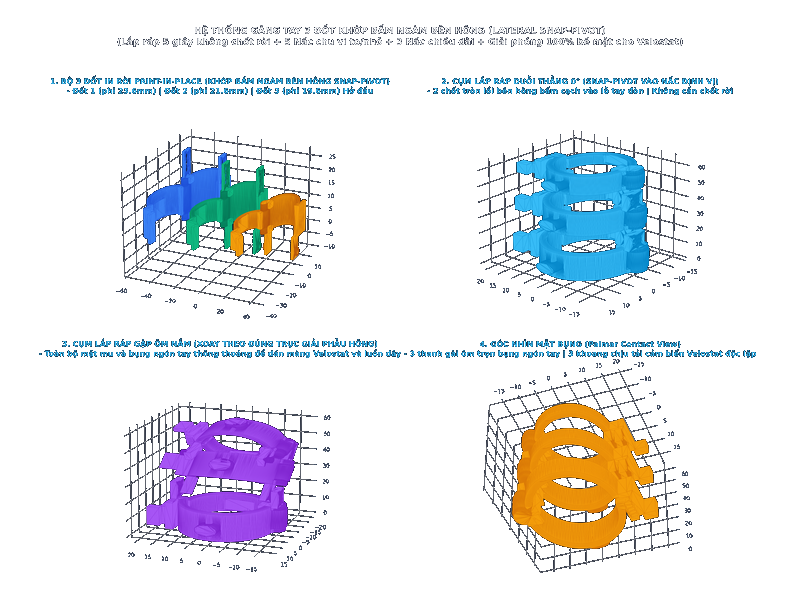
\includegraphics[width=4.6cm, height=2.5cm, keepaspectratio]{assets/splint_3d_transparent.png}\\[4pt]
  {\bfseries\normalsize Khung nẹp 3 ngón in 3D}\\[2pt]
  {\footnotesize Ngàm xoay 2 bản lề tháo mở 1 tay}\\[6pt]
  
  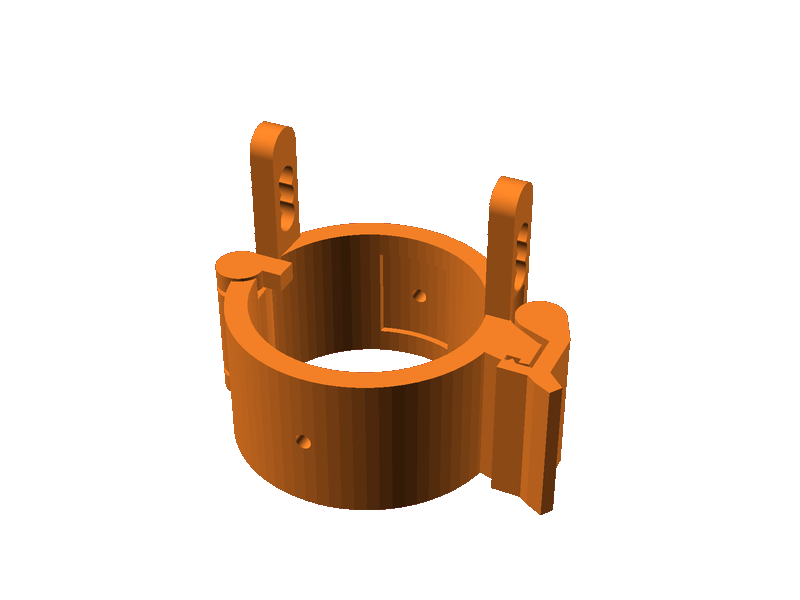
\includegraphics[width=4.2cm, height=1.8cm, keepaspectratio]{assets/mech9_transparent.png}\\[4pt]
  {\bfseries\normalsize 16 Velostat vi sai + 3 Flex}\\[2pt]
  {\small Thu nhận nỗ lực vận động \& Góc gập}
};

\node[tierCard, text width=6.6cm, minimum height=7.2cm, right=72pt of tier2.north east, anchor=north west] (tier3) {
  {\bfseries\Large TẦNG 3: TRỢ LỰC}\\[2pt]
  {\footnotesize\color{black!70} (Actuation Tier)}\\[8pt]
  
  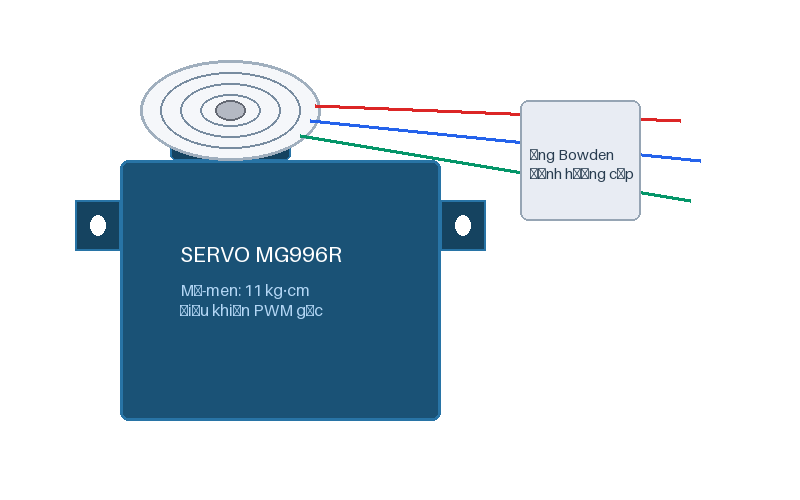
\includegraphics[width=4.8cm, height=2.6cm, keepaspectratio]{assets/servo_spool_assembly.png}\\[6pt]
  {\bfseries\normalsize 3 Servo MG996R \& Tang cáp}\\[2pt]
  {\footnotesize Lực kéo chủ động 11 kg$\cdot$cm trên 3 ngón}\\[8pt]
  
  {\bfseries\normalsize Truyền động cáp Bowden}\\[2pt]
  {\small Trợ lực gập chủ động theo nỗ lực}\\[2pt]
  {\small Nẹp đàn hồi hồi vị đẩy mở ngón}
};

% ==================== 3. TẦNG 4: THỊ GIÁC 3D (ĐẶT PHÍA TRÊN TẦNG 2 CÁCH 50PT) ====================
\node[tierCard, text width=9.6cm, above=50pt of tier2] (tier4) {
  {\bfseries\Large TẦNG 4: THỊ GIÁC 3D \& TÁC VỤ}\\[2pt]
  {\footnotesize\color{black!70} (Vision Pre-Actuation Tier)}\\[6pt]
  
  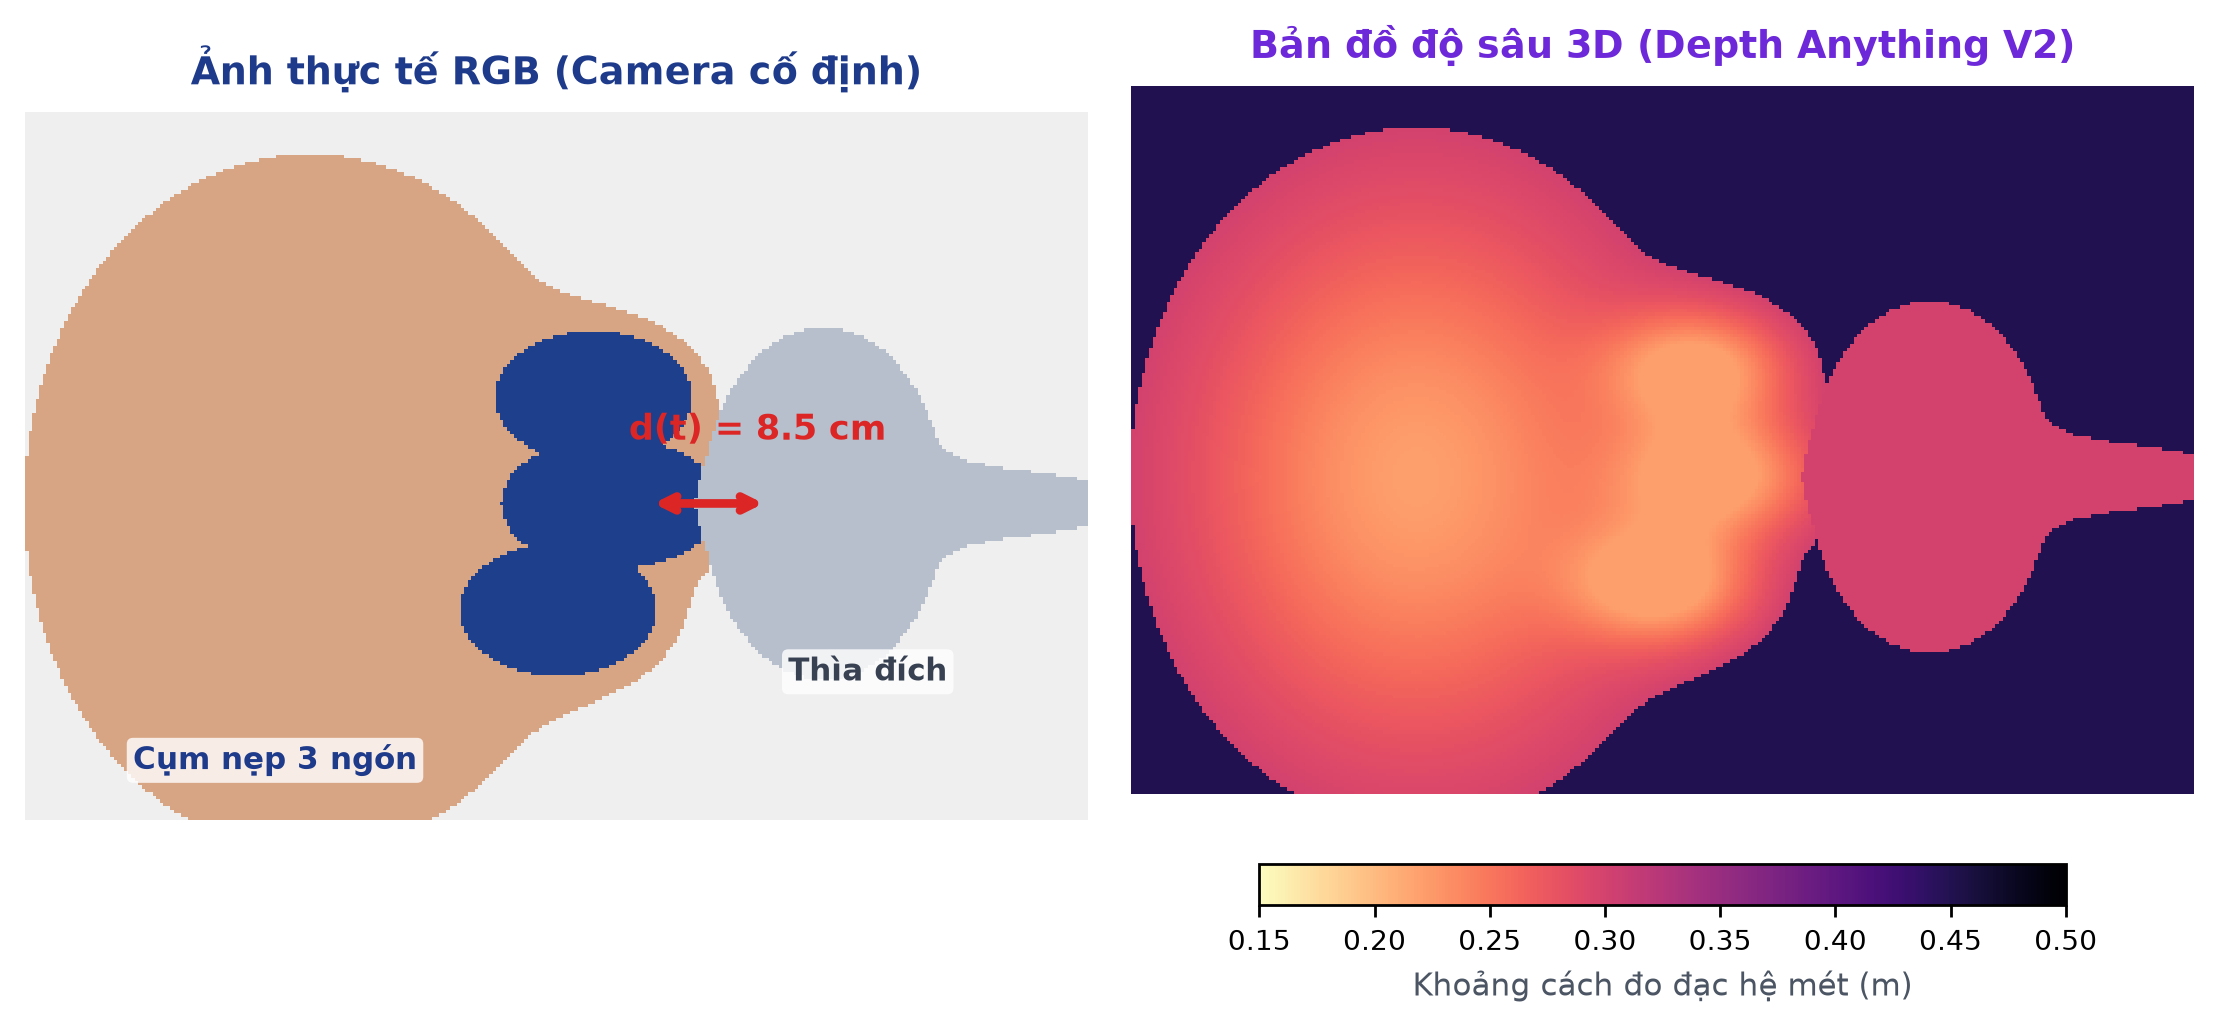
\includegraphics[width=8.0cm, height=2.2cm, keepaspectratio]{assets/depth_anything_scene.png}\\[4pt]
  {\bfseries\normalsize Orange Pi 5 Pro + Depth Anything V2 (3D)}\\[2pt]
  {\small Ước lượng cự ly 3D $d(t)$ \& Thời gian tới tiếp xúc (TTC) đón trước}
};

% ==================== MŨI TÊN KẾT NỐI LUỒNG TÍN HIỆU & ĐIỀU KHIỂN ====================

% Tầng 1 -> Tầng 2: Tín hiệu tương tự 21 kênh
\draw[arrowThick] (tier1.east) -- 
  node[tagText, above=3pt] {Tín hiệu 21 kênh} 
  node[tagText, below=3pt] {Áp lực vi sai \& Góc} 
  (tier2.west);

% Tầng 2 -> Tầng 3: Lệnh điều khiển servo AAN
\draw[arrowThick] (tier2.east) -- 
  node[tagText, above=3pt] {Lệnh servo AAN} 
  node[tagText, below=3pt] {Kéo gập / Nhả duỗi} 
  (tier3.west);

% Tầng 4 -> Tầng 2: Cự ly 3D và TTC đón trước (UART/USB)
\draw[arrowThick] (tier4.south) -- 
  node[tagText, midway] {Khẩu độ \& TTC đón trước (UART)} 
  (tier2.north);

% Tầng 4 -> Tầng 1: Quan sát không gian bài tập
\draw[arrowThick, dashed] (tier4.west) -| 
  node[tagText, pos=0.35, above=3pt] {Quan sát cự ly 3D tay -- thìa} 
  (tier1.north);

% ==================== VÒNG PHẢN HỒI CƠ HỌC (ĐÁY): TẦNG 3 -> TẦNG 1 ====================
\draw[arrowThick] (tier3.south) -- ++(0, -1.2cm) 
  -- node[tagText, fill=white, inner sep=4pt] {Vòng phản hồi cơ học: Cáp Bowden kéo trợ lực gập / Nhả duỗi mở ngón} 
  ($(tier1.south) + (0, -1.2cm)$) -- (tier1.south);

\end{tikzpicture}
\end{document}
